%author: Pedro Pinto; v2.5; jun 2020
\documentclass[11pt,a4paper]{report}
\usepackage{amsmath}
\usepackage{graphicx}
\usepackage{tabularx}
\usepackage{adjustbox}
%\usepackage[colorinlistoftodos]{todonotes}
\usepackage{csquotes}
\usepackage{comment}
\usepackage{imakeidx}
%tabela
\usepackage{multirow}
\usepackage{xcolor}
\usepackage[margin=3cm]{geometry}
\usepackage{hyperref}
\usepackage[toc,acronym,nopostdot,nonumberlist]{glossaries}
\usepackage{titling}
\usepackage{tikzpagenodes}
\usepackage[ddmmyyyy]{datetime}
\usepackage{setspace}
\usepackage{indentfirst}

%para definir a localização das tabelas e imagens em modo strict
%\usepackage{placeins}

% Solving environment subfigure undefined
\usepackage{subcaption}
\captionsetup{compatibility=false}
% Solving environment subfigure undefined


\usepackage{biblatex}
\addbibresource{ref.bib}
\makeglossaries

%colocar aqui variáveis que serão utilizadas no texto:
\newcommand\kbps{\text{\textit{k}bit/s}}
\doublespacing

\begin{document}

\begin{titlepage}
\begin{tikzpicture}[remember picture,overlay,shift={(current page.center)}]
\node[anchor=center,xshift=0cm,yshift=9.5cm,opacity=0.75]{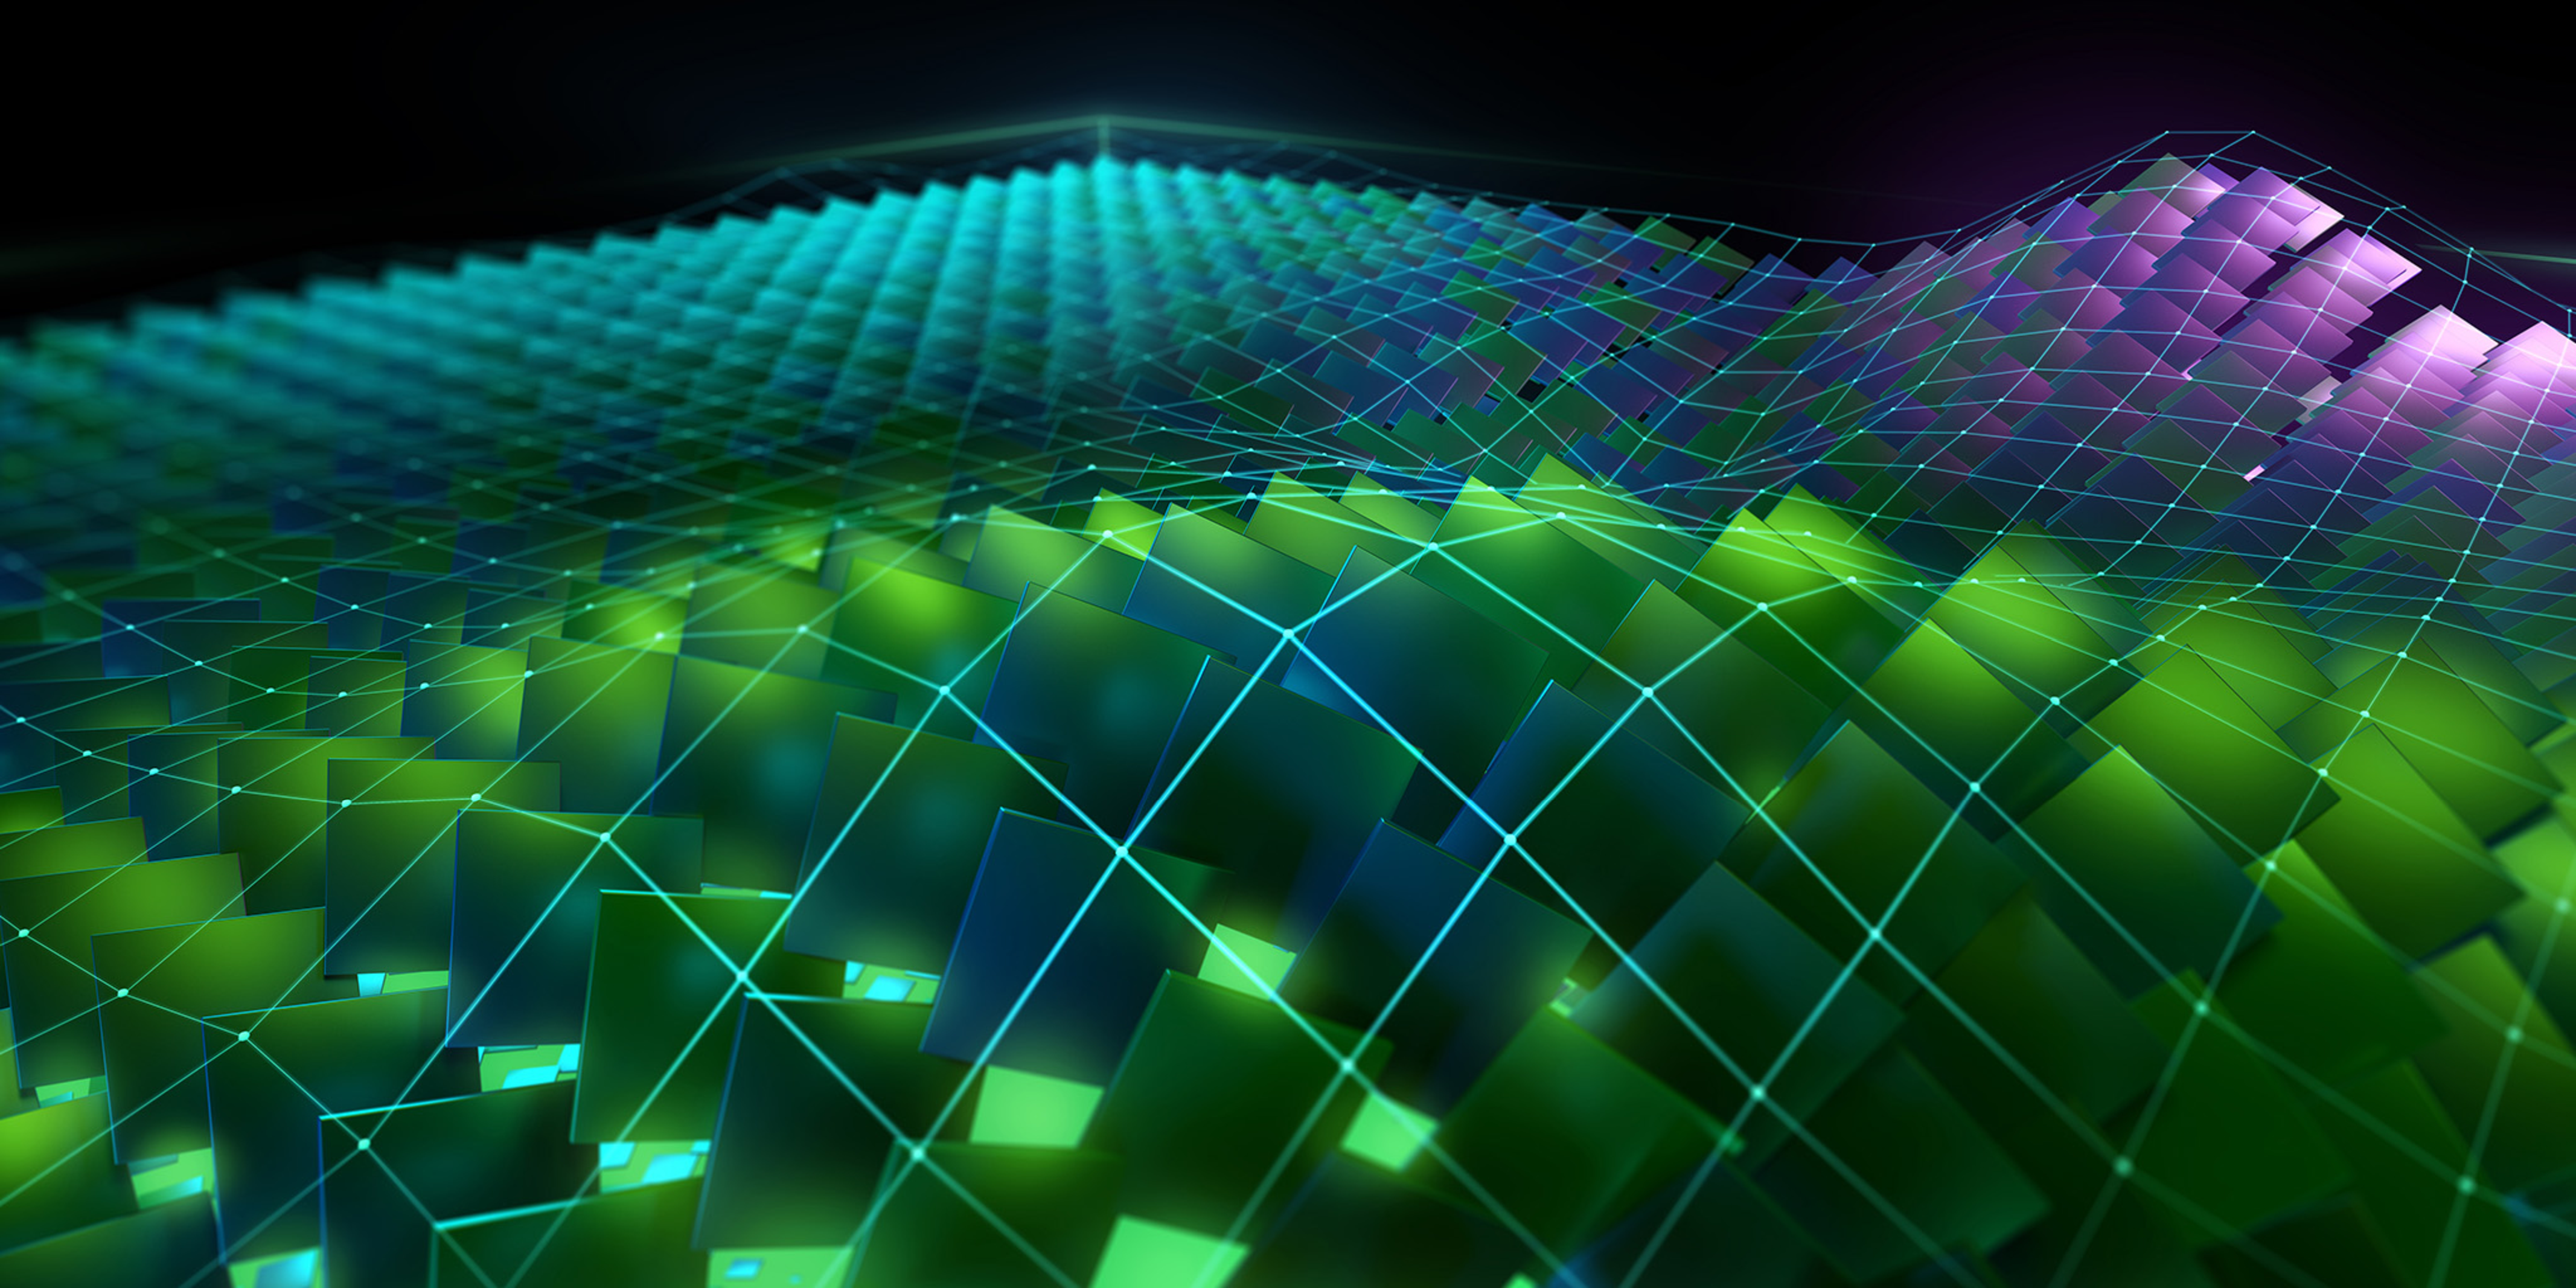
\includegraphics[scale=0.3]{figs/cuda-frontpage.pdf}};
\end{tikzpicture}

\centering
\vspace{10cm}
\huge Classifying CIFAR-10 with Transfer Learning and GPU Acceleration \\
\vspace{3cm}
\large A DD2360 Project\\
%\large a lab assignment report authored by\\
\Large Roderick Karlemstrand\\
\Large KTH Royal Institute of Technology \\

% \large supervised by\\
% %#if Project uncomment
% \large name\\

%#if Internship uncomment following lines
%\large Prof. X (ESTG-IPVC)\\
%\large Name of Company Supervisor (Company X)\\

\vspace{3cm}
%#if Internship uncomment following lines
%\includegraphics[scale=0.35]{figs/ESTG-IPVC.png}

\newdateformat{daymonthyear}{\THEDAY\ \monthname[\THEMONTH], \THEYEAR}
\daymonthyear\today \\
%December, 2019
%\large v2.3
\end{titlepage}

%%%% colocar aqui acrónimos
\newacronym{ersc}{ERSC}{Engenharia de Redes e Sistemas de Computadores}
\newacronym{wn}{WN}{Wireless Network}

%%%%%%%%%%%%%%%%%%%%%%%%%%%%%%%%%%%%%%%%%%%%%%%%%%%%%
\begin{abstract}
%context

%problem

%proposal

%solution

CIFAR-10 is a famous dataset for multiclassification problems. In this project, a Variational Autoencoder is used to classify an unlabeled sub-dataset of CIFAR-10 of 10 000 elements. Next, a small labelled dataset is used to train the classification model. The model is lastly evaluated by a test dataset. The training process takes approximately 30 minutes per epoch with CPU, so that the whole training may take days to finish one experiment. To make the research possible, a GPU accelerated environment was implemented. The results show a speedup by nearly 20 times, and the classification accuracy is around 37\%. \\

\textbf{Keywords:} Image classification, Variational Autoencoder, Deep learning, Transfer Learning, GPU acceleration


\end{abstract}


%insert index
\tableofcontents
\glsaddall
\printglossary[type=\acronymtype]
\printglossary[type=main,title={Glossary},toctitle={Glossary}]
%%%%%%%%%%%%%%%%%%%%%%%%%%%%%%%%%%%%%%%%%%%%%%%%%%%%%

\chapter{Introduction}
\label{chap:introduction}

Computer vision is a field of study in Machine Learning, to give computer programs the ability to see. As for humans, the light reaches the retina and signals are then sent to the brain for further processing. Human brains can connect sight with other senses, like touch, sound or smell. This makes it easy to extract certain things from the sight, to identify them. For example, a child may recognise a bike after seeing a few of them. However, it is not easy for computer programs. The pictures are just like random numbers to them, and it would take thousands of training examples for a Machine Learning model to be able to identify one certain item.


\section{Problem Statement and Motivation}
\label{sec:motivation}

For supervised learning, the dataset has to be labelled and this is often done by humans. It is a very tedious and time-consuming job. Consider also another scenario that for autonomous driving cars, the computer program should be able to identify humans, objects, vehicles and many other things in the environment. And the input data is streaming. It would not be feasible to set labels on every one of these for every single frame. It may be possible to solve the problem in a more efficient way. In this project, a new learning algorithm of Transfer Learning is proposed. A VAE is used to separate the unlabeled training dataset into 10 clusters. And a smalled labelled training dataset is used to help the model associate the clustered learnt with the correct labels. There are no misclassifications (i.e. noises in the dataset). In this way, the model may achieve the same prediction accuracy with the much smaller labelled training dataset. The research questions are:

\begin{itemize}
    \item Is there a more efficient way, VAE, in particular, of teaching computer programs to classify images without large labelled dataset?
    \item How much faster does the training process run with a GPU, specifically Nvidia Tesla P100 16GB?
\end{itemize}


\section{Related Work}

Modelling is widely used in scientific researches. One way of doing it in the field of machine learning is discriminative modelling, which means it will try to predict something give certain observations. For example, giving an image of a cat or a dog, a machine learning model will predict the likelihood of the image being of a cat, or a dog; giving an X-ray image of a tumour, a model will predict if it is benign or malignant. Another way of modelling is called generative modelling. The machine learning model will try to generate some output given certain observations. Generative models may be superior over discriminative models, especially in the problem described above. In this scenario, one can use the generative model of the data to improve classification\cite{kingma2014}.

\section{Objectives}
\label{sec:name}

The objectives of this project are to build a VAE and transfer learning algorithm and to accelerate the training process with GPU.


\chapter{Methods}
\label{cap:method}

The design of the VAE and neural network is presented in this chapter. It also includes the dataset and training process.

\section{Variational Autoencoders}
\label{sec:vae}

An autoencoder is a type of neural network that tries to extract features from the input data and stores it in \textit{codes}. Codes are also known as abstract patterns. This technique forces the neural network to build a system to compress the data. Next, the code is fed into a decoder which tries to re-create the input data. This is called reconstruction \cite{kingma2013auto}. The figure \ref{fig:vae} shows a special type of autoencoders, Variational Autoencoder, whose standard variation and mean value is fixed.

\begin{figure}[h!]
\noindent\makebox[\textwidth]{%
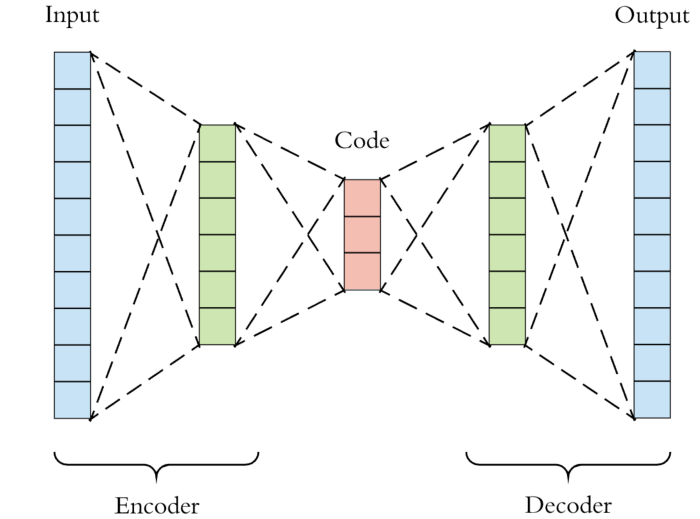
\includegraphics[width=0.6\textwidth]{figs/vae.png}}
\caption{An exampel of a Variational Autoencoder}
  \label{fig:vae}
\end{figure}

\begin{figure}[h!]
\noindent\makebox[\textwidth]{%
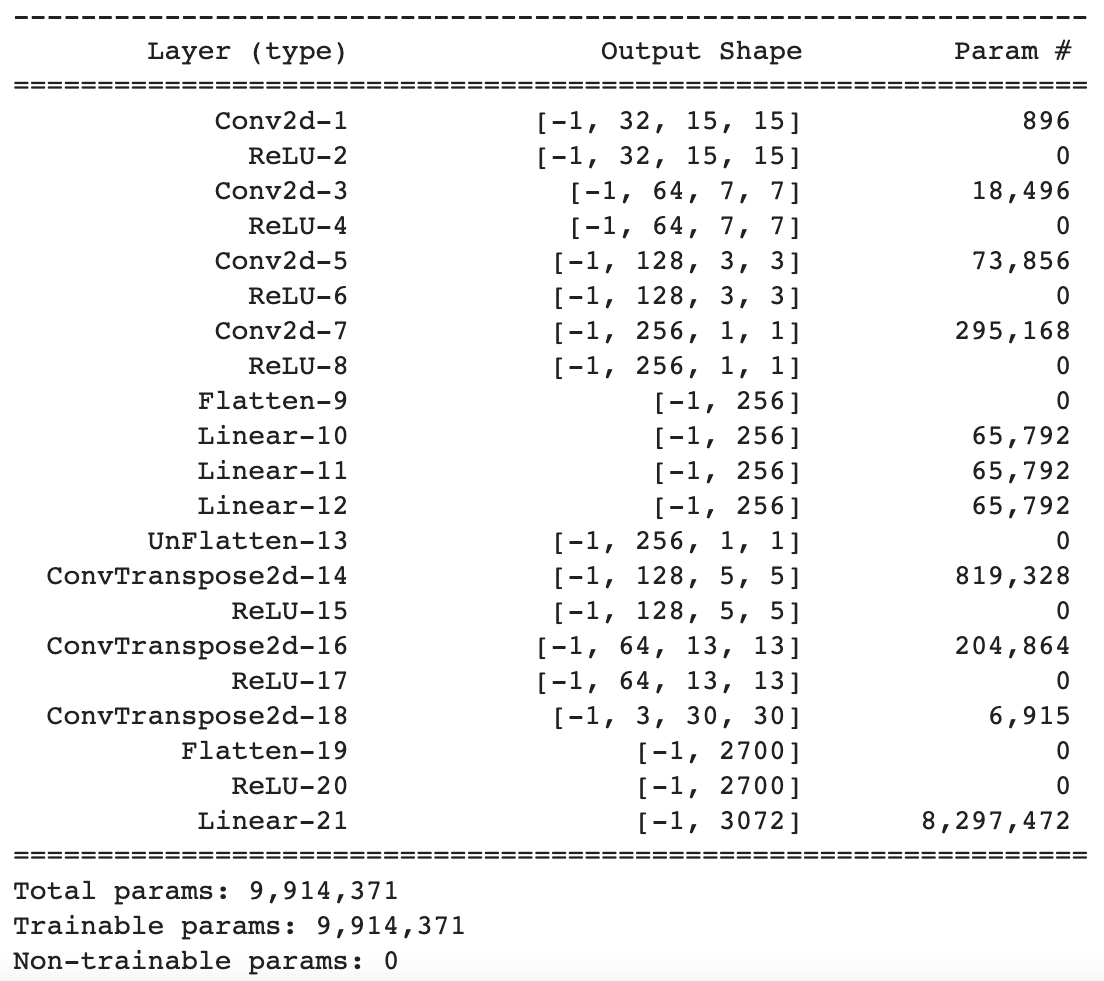
\includegraphics[width=0.8\textwidth]{figs/model.png}}
\caption{An exampel of a Variational Autoencoder}
  \label{tab:model}
\end{figure}

In this project, the architecture of the VAE is designed as table \ref{tab:model}. The input data is images of batch size 32. Each of them has 3 colour channels and for each channel, there are 32x32 pixels. 4 convolution kernels are applied in turn to the input images, with stride size 2 and no paddings. And the activation function is ReLU. The data is then passed into the bottleneck, to force the network to find a pattern. The bottleneck is consist of Linear-10, Linear-11 and Linear-12. For the decoder, everything is reversed. As shown in layer 13 - 20. The Linear-21 will output the generated data into a simple fully connected neural network. It has 2 layers with 100 neurons each, and the output layer has 10 neurons, hence the model will predict the likelihood among 10 different classes.


\section{Dataset}
\label{sec:data}

CIFAR-10 is a famous dataset for solving classification problems. It has 60 000 colour images with resolution 32x32 \cite{cifar10}. This dataset is suitable for researchers who have computers with limited computing power because of the low resolution. Typically in the industry, it would require a computer with dual Xeon processors and 10 graphics cards to do experiments in different design of machine learning models without taking years. In this project, a similar data set is provided by an external sponsor, who prefer rather not to be disclosed. It also has 10 classes \ref{fig:dataset}, by the number of labelled images is only 1 500. There are also 10 000 unlabeled images for unsupervised learning.

\begin{figure}[h!]
    \centering
    \begin{subfigure}[b]{0.4\textwidth}
        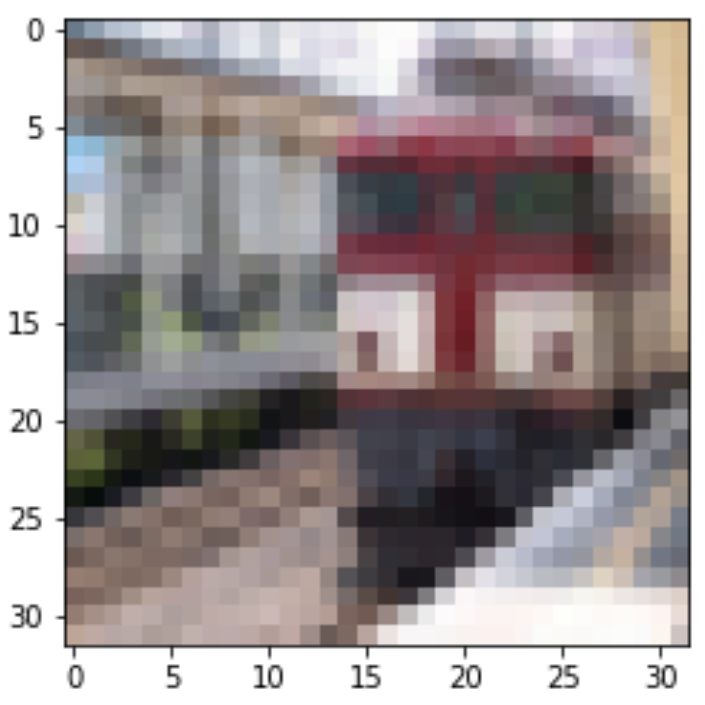
\includegraphics[width=\textwidth]{figs/train.png}
        \caption{A image of a train}
        \label{fig:train}
    \end{subfigure}
    \qquad
    ~ %add desired spacing between images, e. g. ~, \quad, \qquad, \hfill etc.
      %(or a blank line to force the subfigure onto a new line)
    \begin{subfigure}[b]{0.4\textwidth}
        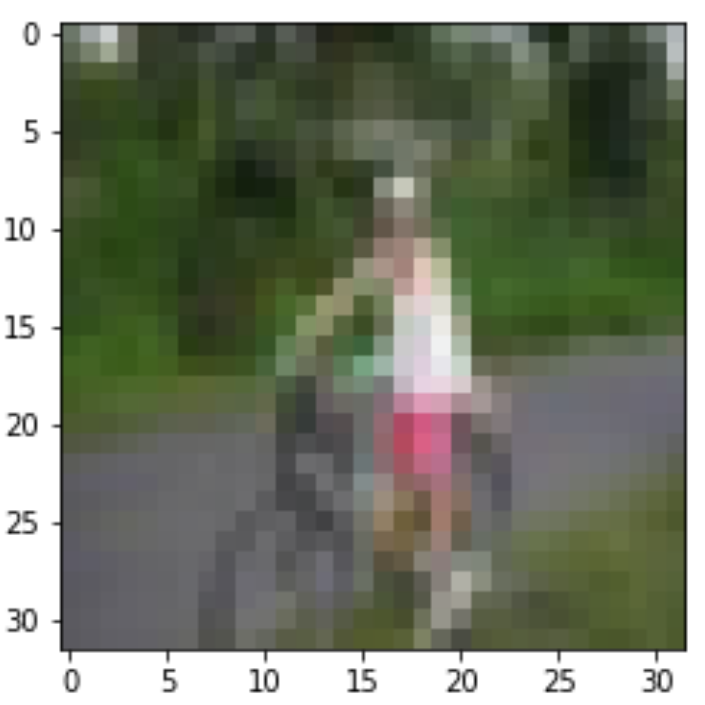
\includegraphics[width=\textwidth]{figs/bike.png}
        \caption{A image of a bicyle}
        \label{fig:bike}
    \end{subfigure}
    \caption{Two examples from the dataset}
    \label{fig:dataset}
\end{figure}


\section{GPU Acceleration}
\label{sec:gpu}

The training of the VAE initially took place on a laptop with an Intel Core i5-7300HQ CPU, and it took about 30 minutes per epoch. Training 200 epochs would take several days. Then the training was tested on another laptop with i7-8750H, which has 6 core, 12 thread. But the temperature went so high and the fans started spinning at high RPMs. So it wasn't an optimal solution. And this is where GPU comes in handy in convolutional neural networks. The training was done using an Nvidia Tesla P100 with 16GB of graphics memory. Small adjustments were made to move the model and input data forward to the GPU.


%%%%%%%%%%%%%%%%%%%%%%%%%%%%%%%%%%%%%%%%%%%%%%%%%%%%%
\chapter{Results and Discussion}
\label{cap:res}

The training of the VAE and classifier went within 30 minutes and successfully. The validation loss went downwards very quickly and settles down after 50 epochs, to as low as 1.9. The prediction accuracy on the test set was up to 37\%, giving randomised 1024 images where the classes are equally distributed. The model is better than random guess and considering the labelled data is only 1 500 images, the aims are reached and in the 10-classification problem, VAE does help to bring up the prediction accuracy.

\begin{figure}[h!]
\noindent\makebox[\textwidth]{%
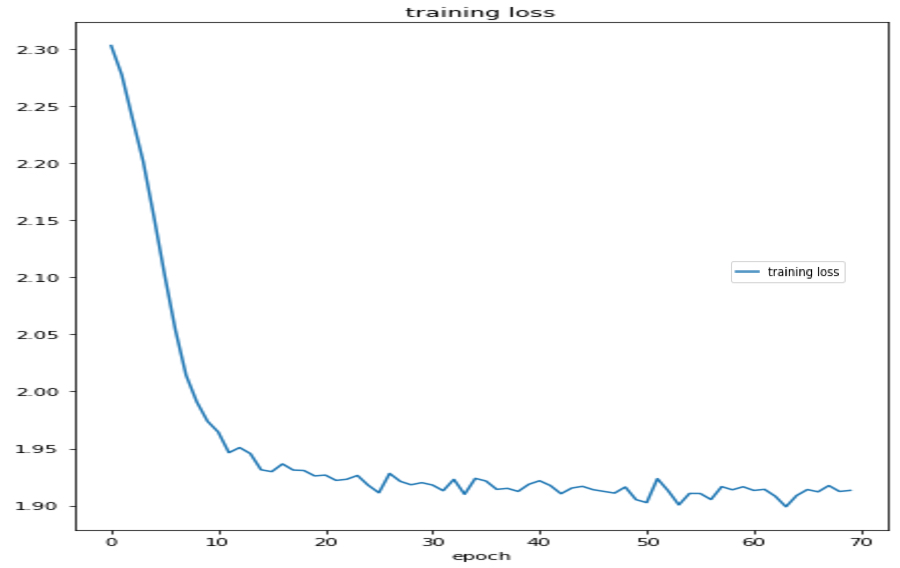
\includegraphics[width=0.6\textwidth]{figs/error.jpg}}
\caption{The Mean Square Error of the classifier on validation set}
  \label{fig:err}
\end{figure}

A comparison between CPU and GPU was also made. The CPU environment was provided by the Center for High-Performance Computing at KTH Royal Institute of Technology. The supercomputer features 128GB of memory and two Intel Xeon E5-2623 v3 3500 MHz processors, each of them has 4 cores and 8 threads. The python program for training the VAE could utilise up to 8 threads. Each epoch has 196 iterations and the training speed was around 1 iteration per second. The whole training process is therefore calculated to be 11 hours \ref{fig:pdc}. Unfortunately, the program caused high CPU usage and was killed by a server administrator before the training was finished. The GPU accelerated environment features 16GB of memory and two virtual cores of a Xeon E5 processor at 2.20 GHz. It has one Nvidia Tesla P100 16GB GPU installed. It only required 9 seconds per epoch and training took less than half an hour \ref{fig:colab}.


\begin{figure}[h!]
\noindent\makebox[\textwidth]{%
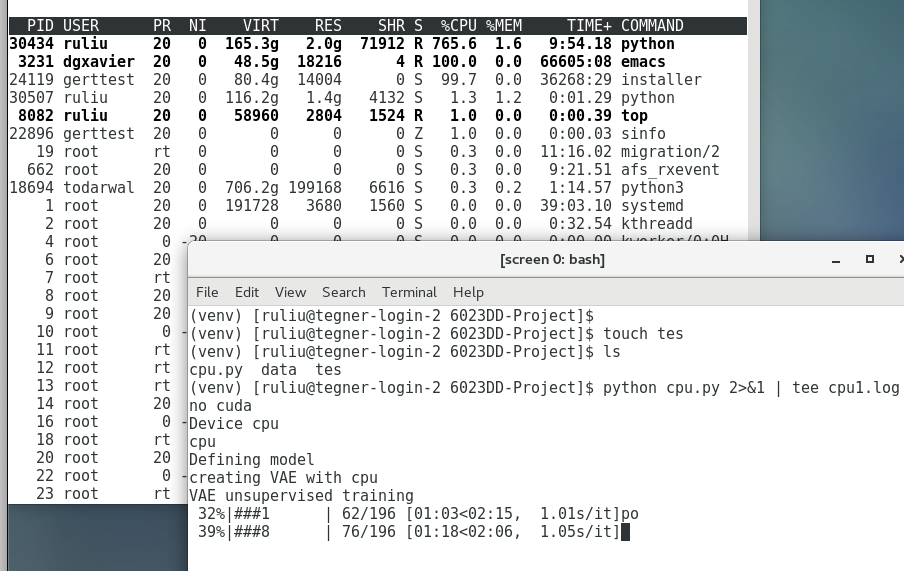
\includegraphics[width=0.9\textwidth]{figs/pdc.png}}
\caption{CPU consumption and time per iteration with CPU}
  \label{fig:pdc}
\end{figure}

\begin{figure}[h!]
\noindent\makebox[\textwidth]{%
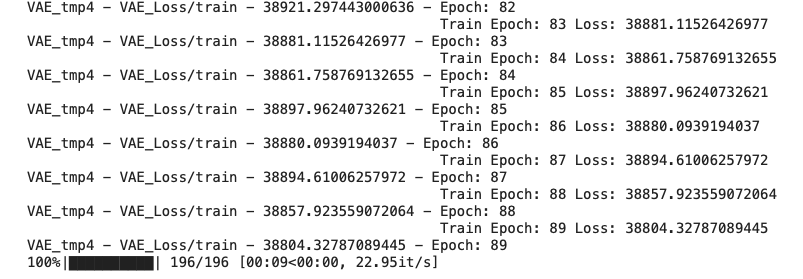
\includegraphics[width=0.9\textwidth]{figs/colab.png}}
\caption{Time per iteration with GPU}
  \label{fig:colab}
\end{figure}

As the classification neural network does not have something remarkable, it may be a good direction in future work. For example, adding dropout layers, experimenting different combinations of neurons in each hidden layer, the number of hidden layers, the activation function in each hidden layer may result in much better prediction accuracy on the test data set. It is also a common practice to add some regularisations into the hidden layers. It can be applied to the kernel, the bias or the output. There are also various regularisations, such as weight decay. By fine-tuning the parameters, it would make it possible to reach the full potential of the VAE architecture. 

There is also a limitation from the dataset. As we can see in figure 1, the picture is very blurry and the picture is about a human and a bicycle. This may confuse the machine learning model. Simple models are not resistant to noises or mislabelling in the training set, hence the performance would suffer from that.

\addcontentsline{toc}{chapter}{References}
\printbibliography[title={References}]

\end{document}
